\begin{figure}[!ht]
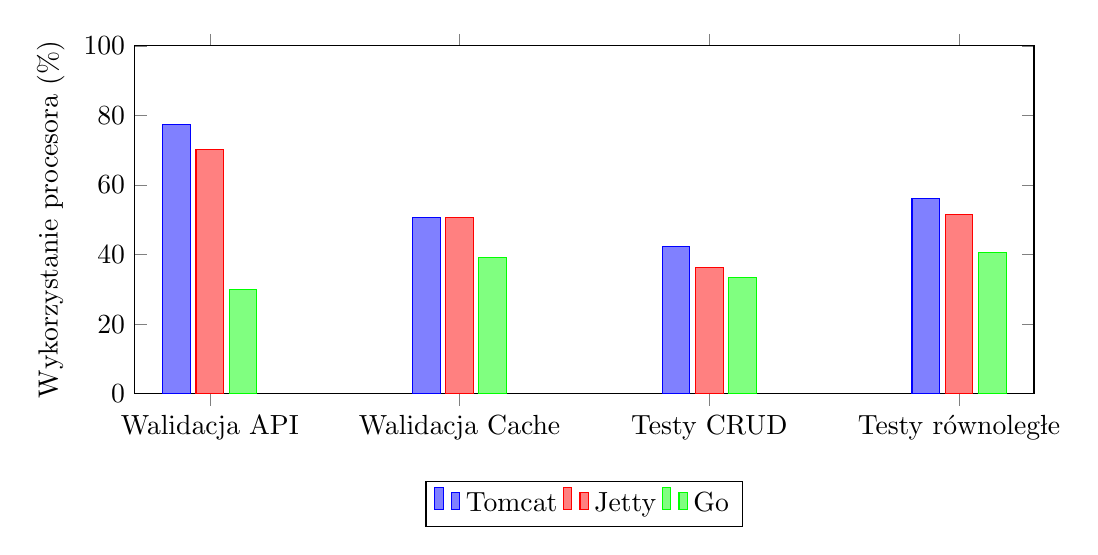
\begin{tikzpicture}
\begin{axis}[
    ybar,
    width=13cm,
    height=6cm,
    legend style={at={(0.5,-0.25)},
      anchor=north,legend columns=-1},
    ylabel={Wykorzystanie procesora (\%)},
    symbolic x coords={Walidacja API, Walidacja Cache, Testy CRUD, Testy równoległe},
    xtick=data,
    ymin=0, ymax=100
    ]

\addplot [blue, fill=blue!50!white] coordinates{ (Walidacja Cache,50.63) (Testy równoległe,56.12) (Walidacja API,77.5) (Testy CRUD,42.38) } ;
\addplot [red, fill=red!50!white] coordinates{ (Walidacja Cache,50.61) (Testy równoległe,51.55) (Walidacja API,70.13) (Testy CRUD,36.32) } ;
\addplot [green, fill=green!50!white] coordinates{ (Walidacja Cache,39.28) (Testy równoległe,40.59) (Walidacja API,29.93) (Testy CRUD,33.31) } ;

\legend{Tomcat,Jetty,Go}
\end{axis}
\end{tikzpicture}
\caption{Wykorzystanie procesora przez aplikacje podczas testów z pustą bazą danych - 100 klientów}
\label{fig:cpu_utilization_100_clean}
\end{figure}



\begin{figure}[!ht]
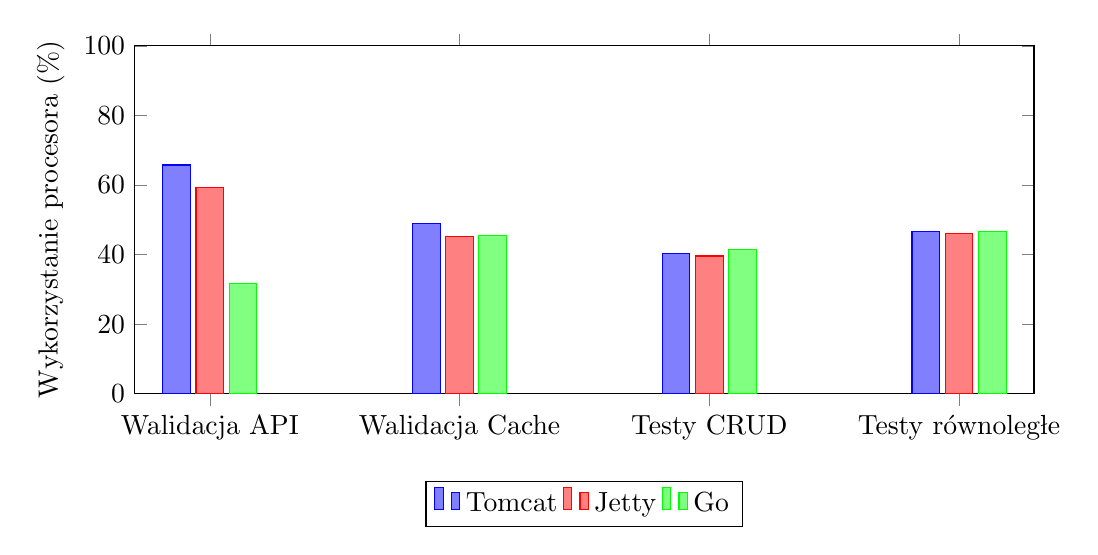
\begin{tikzpicture}
\begin{axis}[
    ybar,
    width=13cm,
    height=6cm,
    legend style={at={(0.5,-0.25)},
      anchor=north,legend columns=-1},
    ylabel={Wykorzystanie procesora (\%)},
    symbolic x coords={Walidacja API, Walidacja Cache, Testy CRUD, Testy równoległe},
    xtick=data,
    ymin=0, ymax=100
    ]

\addplot [blue, fill=blue!50!white] coordinates{ (Walidacja Cache,49.02) (Testy równoległe,46.62) (Walidacja API,65.73) (Testy CRUD,40.25) } ;
\addplot [red, fill=red!50!white] coordinates{ (Walidacja Cache,45.24) (Testy równoległe,46.04) (Walidacja API,59.31) (Testy CRUD,39.6) } ;
\addplot [green, fill=green!50!white] coordinates{ (Walidacja Cache,45.59) (Testy równoległe,46.66) (Walidacja API,31.64) (Testy CRUD,41.36) } ;

\legend{Tomcat,Jetty,Go}
\end{axis}
\end{tikzpicture}
\caption{Wykorzystanie procesora przez aplikacje podczas testów z pustą bazą danych - 250 klientów}
\label{fig:cpu_utilization_250_clean}
\end{figure}